	
	We have given equation as :
	\begin{align}
\left(x-y\right)^2 = x+y+1
\end{align}	
\begin{align}
\implies x^2  -2xy + y^2 -x - y -1 = 0
\label{eq:solutions/41/2/eq1}
\end{align}
The general equation of second degree is given by
\begin{align}
ax^2+2bxy+cy^2+2dx+2ey+f=0 \label{eq:solutions/41/2/eq2}
\end{align}
and can be expressed as
\begin{align}
\vec{x}^T\vec{V}\vec{x}+2\vec{u}^T\vec{x}+f=0 \label{eq:solutions/41/2/eq3}
\end{align}
where
\begin{align}
\vec{V} &= \vec{V}^T = \myvec{a & b \\ b & c}
\\
\vec{u}^T &= \myvec{d & e}
\end{align}

Comparing \eqref{eq:solutions/41/2/eq1} with \eqref{eq:solutions/41/2/eq2}, we get

\begin{align}
\vec{V} &= \vec{V}^T = \myvec{ 1 &  -1 \\ -1 & 1 }
\\
\vec{u}^T &= \myvec{-\frac{1}{2} & - \frac{1}{2}}
\\
f &= -1
\end{align}


Expanding the determinant of V we observe,
\begin{align}
\abs{\vec{V}} = \mydet{1 & -1 \\ -1 & 1} = 0 \label{eq:solutions/41/2/eq10}
\end{align}
Also
\begin{align}
\mydet{\vec{V} & \vec{u} \\ \vec{u}^T & f} = 
\mydet{
1 & -1 & -\frac{1}{2} \\ 
-1 & 1 & -\frac{1}{2} \\ 	
-\frac{1}{2} & -\frac{1}{2} & -1}
\neq 0
\label{eq:solutions/41/2/eq11}
\end{align}

Hence from \eqref{eq:solutions/41/2/eq10} and \eqref{eq:solutions/41/2/eq11} we conclude
that given equation is an parabola.The characteristic equation of $\vec{V}$ is given as
follows,


\begin{align}
\mydet{\lambda \vec{I}-\vec{V}} = \mydet{\lambda -1 & -1 \\ -1 & \lambda - 1} &= 0
\\
\implies \left(\lambda - 1 \right)^2 -1 &= 0
\label{eq:solutions/41/2/eq12}
\end{align}
The eigenvalues are the roots of \eqref{eq:solutions/41/2/eq12} given by
\begin{align}
\lambda_1 = 0, \lambda_2 = 2
\label{eq:solutions/41/2/eq13}
\end{align}
The eigenvector $\vec{p}$ is defined as:
\begin{align}
\vec{V} \vec{p}&= \lambda \vec{p}
\\
\implies \brak{\lambda\vec{I}-\vec{V}}\vec{p} &=0
\end{align}
where $\lambda$ is the eigenvalue.  For $\lambda_1$ = 0,
\begin{align}
\vec{V} \vec{p}&=0
\end{align}
Row reducing $\vec{V}$ yields,
\begin{align}
 \myvec{ 1 & -1 \\ -1 & 1} 
\xleftrightarrow{R_2\leftarrow R_2+R_1} 
\myvec{
	1 &  -1 \\ 0 & 0 
} 
\label{eq:solutions/41/2/eq18}
\end{align}

  Similarly, the eigenvector corresponding to $\lambda_2$ can be obtained as
  
  \begin{align}
  \brak{\lambda_2\vec{I}-\vec{V}}
  = \myvec{ 1 & 1 \\ 1 & 1} 
  \xleftrightarrow{R_2\leftarrow R_2 - R_1}
  \myvec{
  	1 & 1   \\ 0 & 0 
  }
  \label{eq:solutions/41/2/eq19}
  \end{align}
  
  
  

It is easy to verify that 
\begin{align}
\vec{V} &= \vec{P}\vec{D}\vec{P}^{-1}=\vec{P}\vec{D}\vec{P}^T \quad \because \vec{P}^{-1} = \vec{P}^{T} \label{eq:solutions/41/2/eq:solutions/41/ex1/ellipse_spectrum_eq}
\\
\text{or, } \vec{D} &= \vec{P}^T\vec{V}\vec{P}
\end{align}


From equation \eqref{eq:solutions/41/2/eq18} and \eqref{eq:solutions/41/2/eq19}, we have
\begin{align}
\vec{p_1} =  \frac{1}{\sqrt{2}} \myvec{1 \\ 1} 
\text{and},  \vec{p_2} =  \frac{1}{\sqrt{2}} \myvec{1 \\ -1} 
\end{align}
Thus, the eigenvector rotation matrix and the
eigenvalue matrix are 
\begin{align}
\vec{P} &= \frac{1}{\sqrt{2}} \myvec{ \vec{p_1} & \vec{p_2}} = \frac{1}{\sqrt{2}} \myvec{ 1 & 1 \\ 1 & -1} \\
 \vec{D} &= \myvec{0 & 0 \\ 0 & 2} 
\end{align}

\begin{figure}[htb!]	
	\centering	
	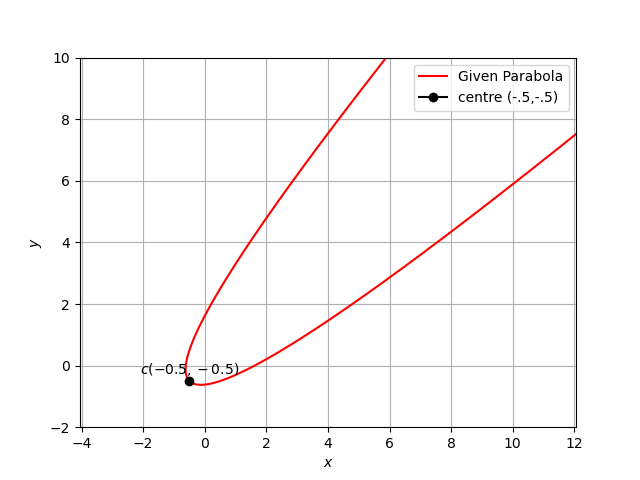
\includegraphics[width=\columnwidth]{./solutions/41/2/parabola.png}	
	\caption{Parabola with the center c}
	\label{eq:solutions/41/2/fig1}	
\end{figure}

The focal length of the parabola is
given by
\begin{align}
\frac{\mydet{2{\vec{u}}^T\vec{p_1}}}{\lambda_2 } = \frac{\sqrt{2}}{2} = \sqrt{2}
\end{align}
and its equation is
\begin{align}
\vec{y}^T\vec{D}\vec{y} = -2 \eta\myvec{1 & 0 }\vec{y}
\end{align}
where,
\begin{align}
\eta = \vec{u}^T\vec{p_1} = - \frac{1}{\sqrt{2}}
\end{align}

\begin{align}
\myvec{\vec{u}^T + \eta\vec{p_1}^T \\ \vec{V}}\vec{c} = \myvec{-f \\ \eta\vec{p_1} - \vec{u}} 
\end{align}
\begin{align}
\implies \myvec{ -1 & -1   \\ 1 & -1 \\ -1 & 1 }\vec{c} = \myvec{1 \\ 0 \\ 0}
\end{align}
Forming the augmented matrix and row reducing
it:


%\begin{align}
%\myvec{-1  &  -1 &  1 \\   1 & -1 &  1 \\  -1 & 1 & 0}  \label{eq:solutions/41/2/2.30}
%\end{align}

\begin{align}
\myvec{-1  &  -1 &  1 \\   1 & -1 &  1 \\  -1 & 1 & 0}  \label{eq:solutions/41/2/2.30}
\xleftrightarrow[]{R_2 \leftarrow R_2+R_1  }
%
\myvec{
-1 & -1 & 1 \\ 0 & -2 & 1 \\ -1 & 1 & 0  
} 
\xleftrightarrow[R_1 \leftarrow -1R_1] {R_3 \leftarrow  R_3 - R_1}  \nonumber  \\
%
\myvec{
1 & 1 & -1 \\ 0 & -2 & 1 \\ 0 & 2 & -1 
}
\xleftrightarrow[]{R_3 \leftarrow R_3 +R_2 } 
%	
\myvec{
1 & 1 & -1 \\ 0 & -2 & 1 \\ 0 & 0 & 0 
} \nonumber   \\
\xleftrightarrow[R_1 \leftarrow R_1 -R_2]{R_1 \leftarrow \frac{R_1}{-2}} 
\myvec{
1 & 0 & -\frac{1}{2} \\ 0 & 1 & - \frac{1}{2} \\ 0 & 0 & 0
}
\end{align}
So,
\begin{align}
\vec{c} = \myvec{ -\frac{1}{2} \\ -\frac{1}{2}  } \label{eq:solutions/41/2/2.31}
\end{align}






